%!TEX TS-program = xelatex
\documentclass[a3paper]{adcv_color}
\usepackage[english]{babel}
\usepackage{multicol}
\usepackage{scrextend}
\usepackage{graphicx}
\usepackage{float}
\setlength{\columnsep}{1cm}
\newenvironment{proyects}[2]{\begin{minipage}{0.8\linewidth}\textbf{#1}
\end{minipage}\begin{minipage}{0.2\linewidth}
    \begin{flushright}
      #2
}{\end{flushright}
  \end{minipage}}
% \newenvironment{proyects}[1]{\begin{minipage}{0.8\linewidth}\textbf{#1}}{\end{minipage}}

\title{Gamaliel-Lopez CV}
\pagestyle{empty}
\adcvname{López Padilla}{Giovanni Gamaliel}{}
\adcvemail{giovannilopez9808}{gmail}{com}
\adcvphone{(+52) 871-278-37-70}
\adcvwebsite{http://resumegglp.herokuapp.com/}{resumegglp.herokuapp.com}
%\adcvdate{}

\begin{document}
\changefontsizes{17.5pt}
\begin{minipage}{0.17\linewidth}
  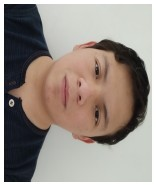
\includegraphics[width=5cm,height=4cm,angle=90]{photo.jpg}
\end{minipage}
\begin{minipage}{0.82\linewidth}
  Me gustan las ciencias y el como puedo abordarlas desde un enfoque matemático con el proposito resolver problemas de una manera óptima mediante la implementación de algoritmos para obtener una mejor comprensión de los fenómenos. De igual manera siento una enorme curiosidad por los sistemas que me rodean y como es que interaccionan con otros.
\end{minipage}\\

\begin{minipage}{0.7\linewidth}
  \section{Habilidades}\\

  \begin{minipage}{0.22\linewidth}
    \begin{flushleft}
      \textbf{S.O.}
      \textbf{Programación}\\
      \textbf{Librerías}\\
      \textbf{Web}\\
      \textbf{Idiomas}
    \end{flushleft}
  \end{minipage}
  \begin{minipage}{0.78\linewidth}
    \begin{flushleft}
      Windows, MacOs, Linux (distribuciones Debian)\\
      Python, Fortran, LaTeX, Java, Julia, C\\
      Numpy, Matplotlib, Pandas, Scipy, Flask, Qiskit\\
      CSS, HTML5, Javascript\\
      Español, ingles
    \end{flushleft}
  \end{minipage}
\end{minipage}
\begin{minipage}{0.29\linewidth}
  \vspace{-1.4cm}
  \section{Educación}\\

  \textbf{Licenciatura en física}\\
  Universidad Autónoma de Nuevo León
\end{minipage}\\

\section{Cursos}

\begin{minipage}{0.85\linewidth}
  \textbf{Qubit x Qubit semestre 1 y 2}\\
  \textbf{Ecuaciones en diferenciales parciales desde la teoría a las aproximaciones numéricas}\\
  \textbf{Qiskit Globar Summer School, IBM}
\end{minipage}
\begin{minipage}{0.15\linewidth}
  %\vspace{-0.cm}
  \begin{flushright}
    agosto 2020\\
    agosto 2020\\
    julio 2020
  \end{flushright}
\end{minipage}\\

\section{Proyectos personales}
\begin{multicols}{2}
  \begin{proyects}{Localización y conteo de incendios en la de Santiago, Nuevo León}{marzo 2021}
  \end{proyects}

  Proyecto actual

  \begin{proyects}{Análisis de parámetros atmosféricos sobre Área Metropolitana de Monterrey en el periodo 2015-2020}{enero 2021}
  \end{proyects}

  En proceso de publicación

  \begin{proyects}{Estimación de los tiempos de exposición solar para la producción de la Pre vitamina D en Rosario, Argentina}{diciembre 2020}
  \end{proyects}

  En proceso de publicación

  \begin{proyects}{Análisis en la tendencia del índice UV en la Ciudad de México en el periodo 2001-2019}{octubre 2020}
  \end{proyects}

  En proceso de publicación

  \begin{proyects}{Localización de incendios en el Delta del río Paraná}{agosto 2020}
  \end{proyects}

  \href{https://github.com/giovannilopez9808/Posters_templates/blob/master/Informe\%20IFIR/Focos\%20de\%20incendio\%20en\%20las\%20islas\%20del\%20Paran\%C3\%A1\%20\%20frente\%20a\%20Rosario\%20\%20(Piacentini\%2C\%20Ipi\%C3\%B1a\%2C\%20Lopez-Padilla\%2C\%20Bolmaro)\%20(Piacentini).pdf}{\textbf{Informe entregado al gobierno de Rosario, Argentina}}

  \begin{proyects}{Cálculo de los tiempos de exposición solar para el tratamiento de Psoriasis en la Ciudad de México}{agosto 2020}
  \end{proyects}

  \href{https://github.com/giovannilopez9808/Posters_templates/blob/master/2020/CNF/TES/main.pdf}{\textbf{Poster}}, \href{http://tes-v1.herokuapp.com/}{\textbf{Plataforma}}

  \begin{proyects}{Análisis de las irradiancias UVA y eritémica medidas por el Sistema Monitoreo atmosférico de la Ciudad de México}{octubre 2019}
  \end{proyects}

  \href{https://github.com/giovannilopez9808/Posters_templates/blob/master/2019/AFA/Analisis\%20indice\%20UV/Analisis\%20de\%20irradiancia.pdf}{\textbf{Poster}}

  \begin{proyects}{Estudio de la irradiancia solar con dos modelos de transferencia radiativa}{agosto 2019}
  \end{proyects}

  \href{https://github.com/giovannilopez9808/Posters_templates/tree/master/2019/CNF/Transferencia\%20radiativa}{\textbf{Poster}}
\end{multicols}
\begin{minipage}{1\linewidth}
  \hspace*{-4cm}
  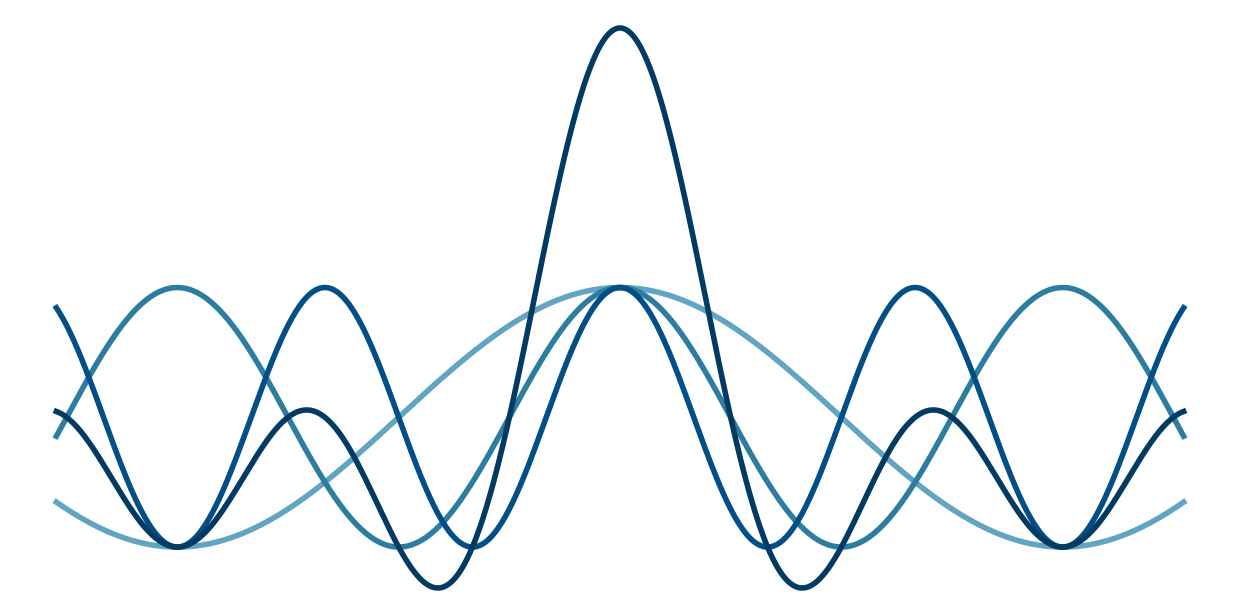
\includegraphics[height=4cm,width=33cm]{image.png}
\end{minipage}
\end{document}
